\documentclass[]{article}

%opening
\title{4F13 Probabilistic Machine Learning - Gaussian Processes}
\author{Lawrence Tray \\ St John's College}

%packages
\usepackage[margin=0.5in]{geometry}
\usepackage{graphicx}
\usepackage{amsmath}
\usepackage{amssymb}
\usepackage{hyperref}
\usepackage{caption}
\usepackage{subcaption}
\usepackage{parskip}

%package setup
\graphicspath{{./img/}}
\DeclareMathOperator*{\argmax}{arg\,max}
\DeclareMathOperator*{\argmin}{arg\,min}

%custom commands
\newcommand{\dft}{\mathcal{F}}
\newcommand{\idft}{\mathcal{F}^{-1}}
\newcommand{\Xcal}{\mathcal{X}}
\newcommand{\Ncal}{\mathcal{N}}
\newcommand{\cmplx}{\mathbb{C}}
\newcommand{\Lcal}{\mathcal{L}}
\newcommand{\figwidth}{0.6\linewidth}

%section numbering
\renewcommand{\thesubsection}{\thesection.\alph{subsection}}

\begin{document}

\maketitle

\begin{abstract}
\end{abstract}

\section{Introduction}

\section{Questions}
\subsection{Squared Exponential Covariance Function}

We start with a simple squared exponential (SE) covariance function. As we start by working in one dimension this is necessarily isotropic. The covariance function is given by:

\begin{equation}
k(x, x') = \nu^2 \exp\left\{- \frac{(x-x')^2}{2l^2}\right\}
\label{eqn:covSEiso}
\end{equation}

The hyperparameters are $\nu$ and $l$ which control the baseline variance level and length scale of variation respectively. We load in the training data from \textit{`cw1a.mat'} and train a GP model, with zero mean and covariance function given by equation \ref{eqn:covSEiso}. We train the model by minimising the negative log marginal likelihood (denoted $\Lcal$). Table \ref{tab:hyp-opt} scenario A shows the how the parameters are optimised.

\begin{table}[!h]
\centering
\begin{tabular}{c | c c | c c}
	\textbf{Parameter} & \textbf{A Initial} & \textbf{A Final} & \textbf{B Initial} & \textbf{B Final} \\ \hline
	$\log l$           & -1                 & -2.054           & -0.45              & 2.085            \\
	$l$                & 0.368              & 0.128            & 0.638              & 8.045            \\
	$\log \nu$         & 0                  & -0.109           & 0                  & -0.363           \\
	$\nu$              & 1                  & 0.897            & 1                  & 0.696            \\
	$\Lcal$            & 0                  & -2.139           & 0                  & -0.411          
\end{tabular}
\caption{Parameter optimisation (log values included for reference as reported by gpml toolbox)}
\label{tab:hyp-opt}
\end{table}

This yields a predictor as in figure \ref{fig:1a}. The 95\% error bound is computed by $[\mu(x) - 2\sigma(x), \mu(x) + 2\sigma(x)]$. In other words, as $y \sim \Ncal(\mu(x), \sigma(x)^2)$, there is a 95\% chance of $y$ falling within two standard deviations of the mean (all evaluated at a specific $x$).

\begin{figure}[!h]
	\begin{subfigure}{0.5\linewidth}
		\centering
		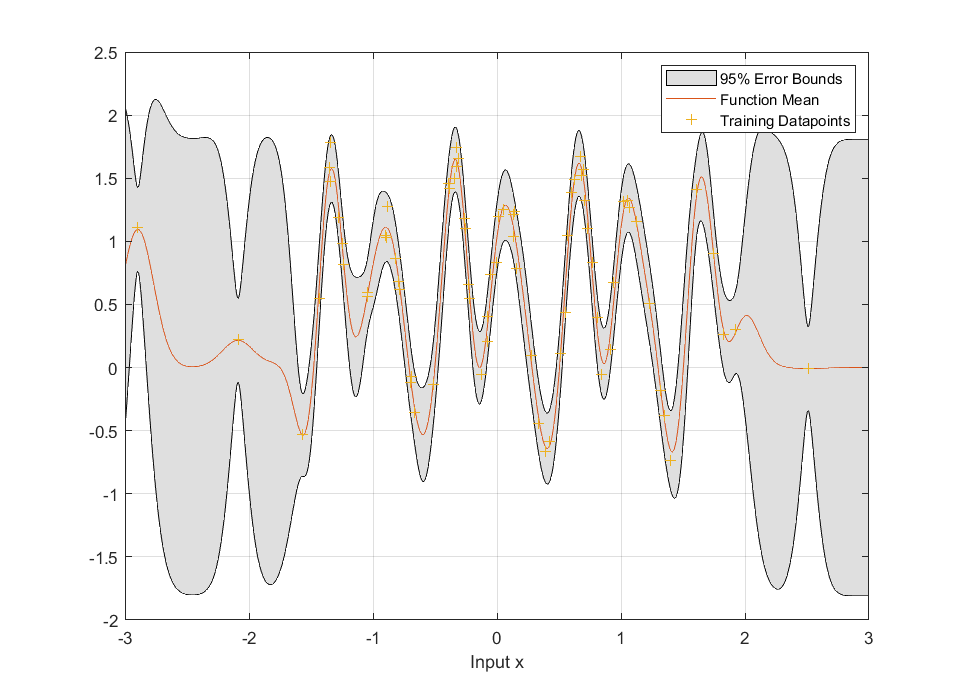
\includegraphics[width=\linewidth]{1a}
		\caption{Basic hyperparameter initialisation}
		\label{fig:1a}
	\end{subfigure}
	\begin{subfigure}{0.5\linewidth}
		\centering
		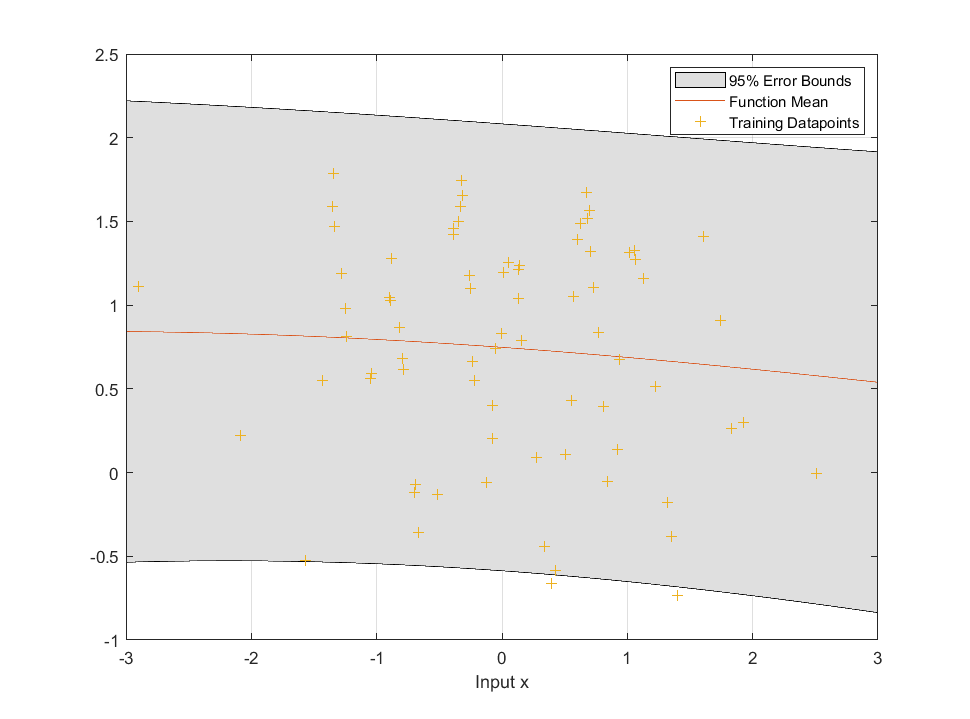
\includegraphics[width=\linewidth]{1b}
		\caption{Alternative hyperparameter initialisation}
		\label{fig:1b}
	\end{subfigure}
	\caption{Squared Exponential covariance Gaussian Process trained on data}
	\label{fig:1}
\end{figure}

We see that the error bars are always centred on the mean and that they have small standard deviations for regions in which we have many datapoints observed. This makes intuitive sense as we cannot make confident predictions in areas where the training data is sparse (such as for $|x| \geq 3$). The hyperparameters do not change enormously form the optimisation. We have that the length scale of variation $l$ shrinks slightly to 0.128 - which agrees with the length scale of variation in the dataset. The scale factor $\nu$ also shrinks slightly to 0.897 as the model is able to match the data quite accurately.

\subsection{Hyperparameter Initialisation}

However, the optimisation only finds a local minimum of the negative log-likelihood $\Lcal$. Therefore, a different intilisation of the hyperparameters can yield different results. This is illustrated in scenario B of table \ref{tab:hyp-opt}. It was found that $\log l = -0.45$ was a critical point. Any setting of $\log l $ above this would converge to the case-B optimum; anything below converges to the original case-A optimum. Varying $\nu$ only seemed to change the position of this critical point but would not converge to an altogether different solution.

 


\subsection{Periodic Covariance Function}

\begin{figure}[!h]
	\centering
	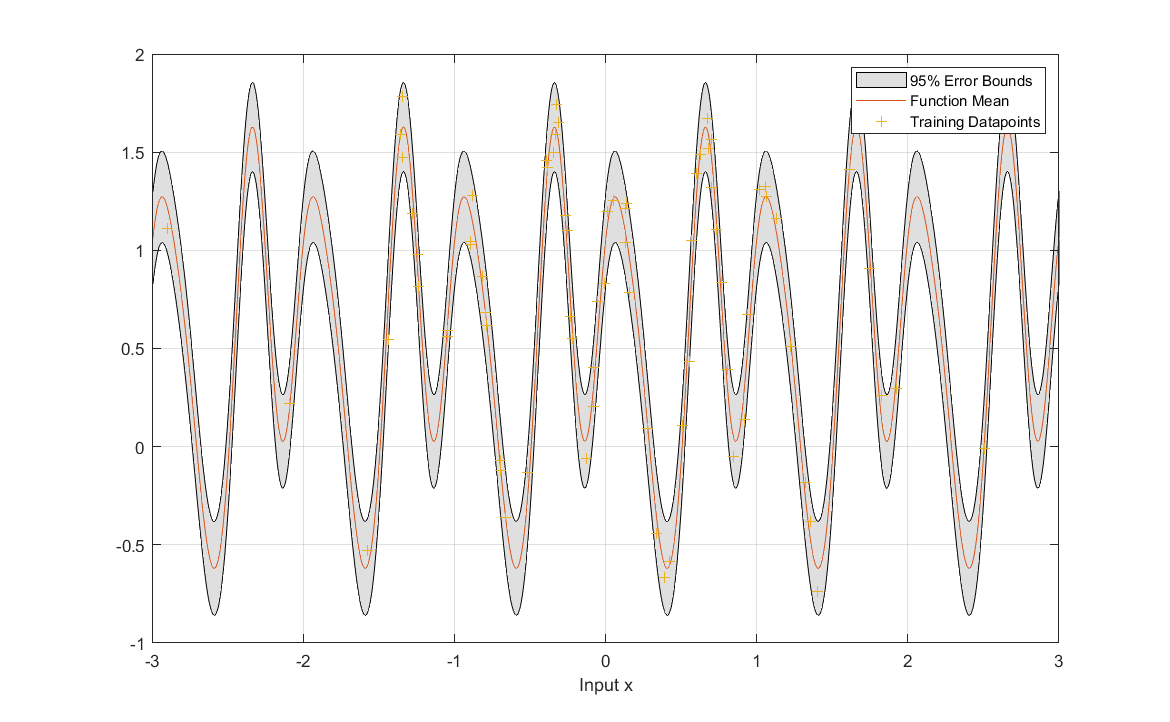
\includegraphics[width=\figwidth]{1c}
	\caption{Periodic covariance GP on same training data}
	\label{fig:1c}
\end{figure}

\subsection{Cholesky Decomposition}

\begin{figure}[!h]
	\centering
	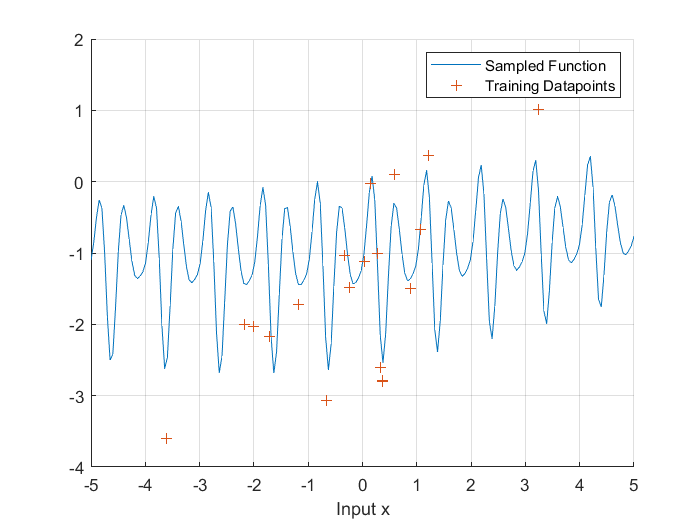
\includegraphics[width=\figwidth]{1d}
	\caption{Trained GP with initial hyperparameter settings}
	\label{fig:1d}
\end{figure}

\subsection{Model Comparison}

\begin{figure}[!h]
	\begin{subfigure}{0.5\linewidth}
		\centering
		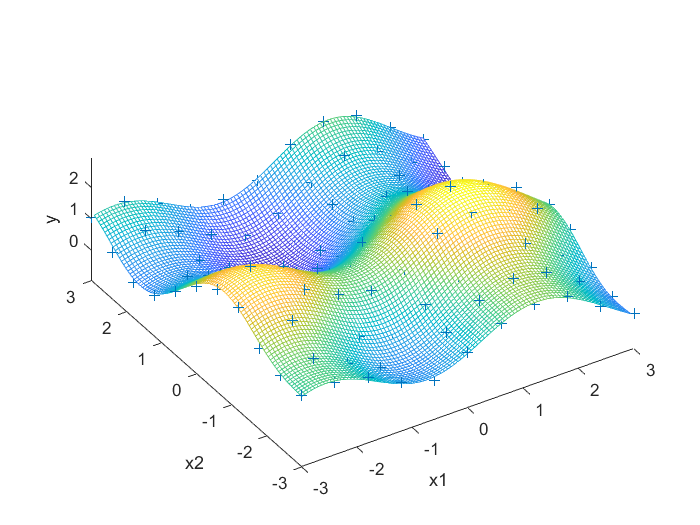
\includegraphics[width=\linewidth]{1e1}
		\caption{Basic covariance function: single covSEard model}
		\label{fig:1e1}
	\end{subfigure}
	\begin{subfigure}{0.5\linewidth}
		\centering
		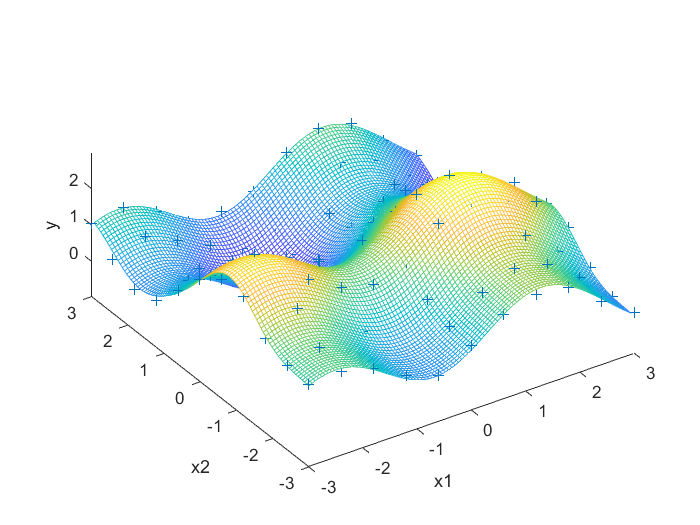
\includegraphics[width=\linewidth]{1e2}
		\caption{Additive covariance function: two covSEard model}
		\label{fig:1e2}
	\end{subfigure}
	\caption{Comparison of two covariance function fits on training data}
	\label{fig:1e}
\end{figure}

\begin{figure}[!h]
	\begin{subfigure}{0.5\linewidth}
		\centering
		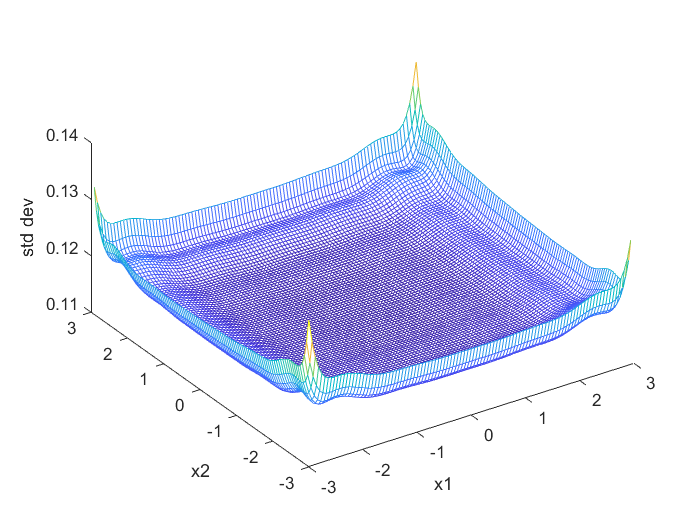
\includegraphics[width=\linewidth]{1e1b}
		\caption{Basic covariance function: single covSEard model}
		\label{fig:1e1}
	\end{subfigure}
	\begin{subfigure}{0.5\linewidth}
		\centering
		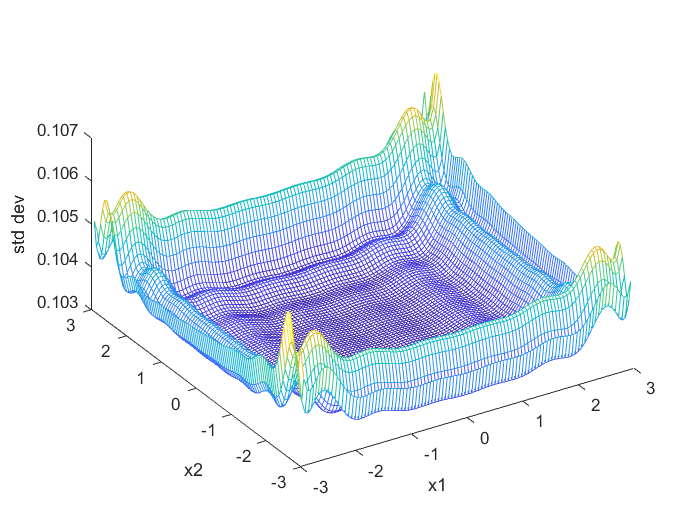
\includegraphics[width=\linewidth]{1e2b}
		\caption{Additive covariance function: two covSEard model}
		\label{fig:1e2}
	\end{subfigure}
	\caption{Comparison of standard deviation for }
	\label{fig:1e}
\end{figure}


\end{document}
